\documentclass[11pt,conference,onecolumn]{IEEEtran}
%\documentclass[11pt,draft,onecolumn]{IEEEtran}
%\IEEEoverridecommandlockouts
% The preceding line is only needed to identify funding in the first footnote. If that is unneeded, please comment it out.
\usepackage{cite}
\usepackage{amsmath,amssymb,amsfonts}
\usepackage{algorithmic}
\usepackage{graphicx}
\usepackage{subcaption}
\usepackage{textcomp}
\usepackage{xcolor}
\usepackage{tabularx}
\usepackage{enumitem}
\usepackage{multirow}
\usepackage[textwidth = 155mm]{geometry}
\usepackage{url}
\usepackage{hyperref}
\hypersetup{colorlinks=true,urlcolor=cyan}
\setlist[itemize]{align=parleft, left=0pt..1em}
\setlength{\textfloatsep}{6pt}
\setitemize{leftmargin=*, align=parleft}
%\overfullrule=1mm
\begin{document}

\title{AI4Agile Summary Report - Team Katara}

\author{\IEEEauthorblockN{Phong Bach, Emily Cawlfield, Nain Galvan, Aric Monary}
\IEEEauthorblockA{\textit{School of Electrical Engineering and Computer Science} \\
\textit{Washington State University}\\
Everett, USA 98201 \\
phong.bach, emily.cawlfield, nain.galvan, aric.monary@wsu.edu}
}
\maketitle
\section{Introduction}
AI4Agile is an add-on application built for Jira Software Cloud \cite{jira2}, made to assist software development teams in agile environments in streamlining user story refinement. The application utilizes Artificial Intelligence (AI) to power processes that refine user stories from epics into tasks. It offers AI-based smart suggestions of requirement work items with different levels of details: epics, user stories, and tasks. Finally, the application provides an integrated tool that allows users to visualize the explicit and implicit relationships among the requirements. Team Katara from Washington State University Everett submits this report for the ICSE SCORE 2021 competition. 

The rest of the report is organized as follows. Section \ref{background} outlines preliminary background information of the app, the stakeholders, and the team's development process. Section \ref{requirement} summarizes the requirements modeling, goal-oriented acquistion and decomposition. Section \ref{design} and \ref{implementation} outline the design and implementation of the tool respectively, while the latter expanded on detailed changes made transitioning from initial design to the final implementation. Section \ref{demo} demonstrates the primary functionalities of the tool via walkthroughs of two use cases, as well as the work done for testing. Lastly, Section \ref{conclusion} reflects on the outcome of the project and explores future prospects of the project. 

\section{Background and Process}
\label{background}
\subsection{Project Scope}
\label{scope}
The team chose the project “AI4Agile: Developing AI-enabled tool support for user story refinement in JIRA” for our participation in the SCORE 2021competition. The project is sponsored by Dr. Hoa Khanh Dam from University of Wollongong in Australia. It stemmed from Dr. Dam's research in the intersection of Software Engineering and Artificial Intelligence \cite{dam1,dam2,dam3}. 

The project proposed four primary requirements \cite{proposal}:

\begin{enumerate}
	\item Recommend user stories that are decomposed from an epic.
	\item Recommend smaller user stories to be split from bigger user stories.
	\item Recommend subtasks derived from a user story.
	\item A visualization (e.g. a graph) of epics, user stories and tasks, and their relationships.
\end{enumerate}

In addition, the application must be integrated and easily deployed into the platform of Atlassian’s Jira software, a widely used software project management tool that provides a marketplace for add-on applications \cite{jira1}. 

\subsection{Teams and Stakeholders}
We entered the SCORE competition upon recommendation by our faculty advisor Dr. Bolong Zeng. The four team members are all senior students in the Software Engineering major at Washington State University, Everett, USA. We complete the project as part of our Software Requirement and Senior Design Capstone courses, and we name ourselves Team Katara. \footnote{As part of this year's theme of our Senior Design Capstone projects (\emph{Avatar: the Last Airbender}).} 

The team chose AI4Agile from the list since the team were most interested in working with AI. The idea of intersecting AI with Software Engineering (SE) was also intriguing, particularly for four Software Engineering major students. The project is essentially a meta-project on SE, as we would be developing an SE tool that helps with the SE process, while conducting our own SE process. 

The team enlisted the help of several faculty and industry mentors/advisors. Dr. Zeng is the faculty advisor who supervises the team's process and review our work products. As the team had no prior experience with AI and Natural Language Processing (NLP), we asked for advice from Prof. Jeremy Thompson, whose main expertise is in these fields. We also contacted the SCORE sponsor for AI4Agile Dr. Dam as soon as the team started working on the project. Dr. Dam provided us with his previous research and publications, from which AI4Agile was born, as well as sample data that he used in the past. 

As the project is a tool for software developers, we were fortunate to have Skip Baccus, a senior project manager from Microsoft, who agreed to fulfill the role as a domain expert. Throughout the project, he worked with us both as a mentor and as a stand-in for potential client. All people mentioned above rounded up the stakeholders in the project. Team member Aric Monary served as the team liaison to coordinate communications among all involved parties.

\subsection{Team Process}
We adopted an agile process for ourselves throughout the project. The members met a minimum of 2 times per week, working on both documentation and implementation tasks. The meetings led into the scrum meeting with our business mentor every Tuesday, where we debriefed the mentor on our progress on features, and solicited feedback from his perspective. In between these meetings, the team worked on their own assignments, while the faculty advisor reviewed our documentations. Figure \ref{fig:acd} shows the major activities of the team on a regular basis. Our approach emphasizes heavily on the quick feedback turn-arounds and frequent iteration loops. 

\begin{figure}
\centering
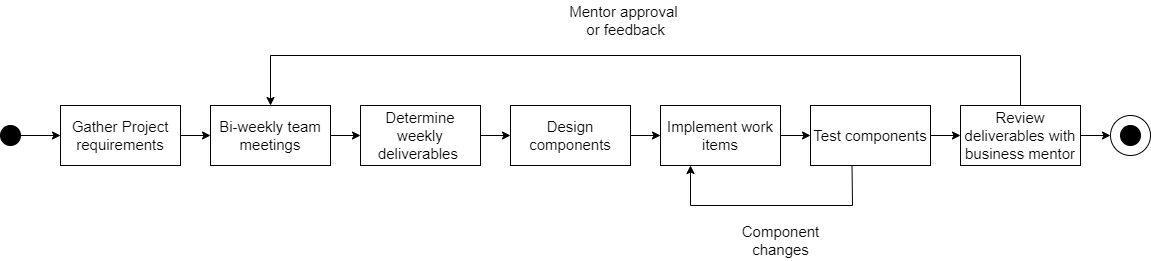
\includegraphics[width=\textwidth,keepaspectratio]{./figure/ActivityDiagram.png}
\caption{Activity Diagram outlining the SE process}
\label{fig:acd}
\end{figure}

The team started by studying Dr. Dam's papers, mainly \cite{dam1}, and brainstorming concepts that we considered vital to the project. We then split into doing research on various key issues, such as Jira API, NLP, and more according to individual strengths and preferences. Meanwhile, the entire team participated in regular requirement gathering sessions with the mentor to refine the initial scope of the project. Throughout the process we have obtained key understanding on the agile process itself, and how the tool can best assist within the project scope. The requirements are presented in more details in Section \ref{requirement}. As we were finalizing the necessary major features, the team simultaneously started early coding to experiment with implementation based on our earlier research. 

The development effort mainly consists of two parts: AI and UI components.  The AI components were of high priority for the majority of the project. Three members each focused on one of the three primary features, while the fourth member focused on building UI for the visualization tool. As the project came to a close, we moved the UI portion as top priority as AI development was completed. As our final milestone, we demonstrated the functional prototype of the tool to our stakeholders by conducting walkthroughs of major use cases. Fig. \ref{fig:timeline} presents the project timeline, with key work tasks and dates noted. Fig. \ref{fig:responsibility} provides an overview of responsibility assignments for functionalities of the add-on.

\begin{figure}
\centering
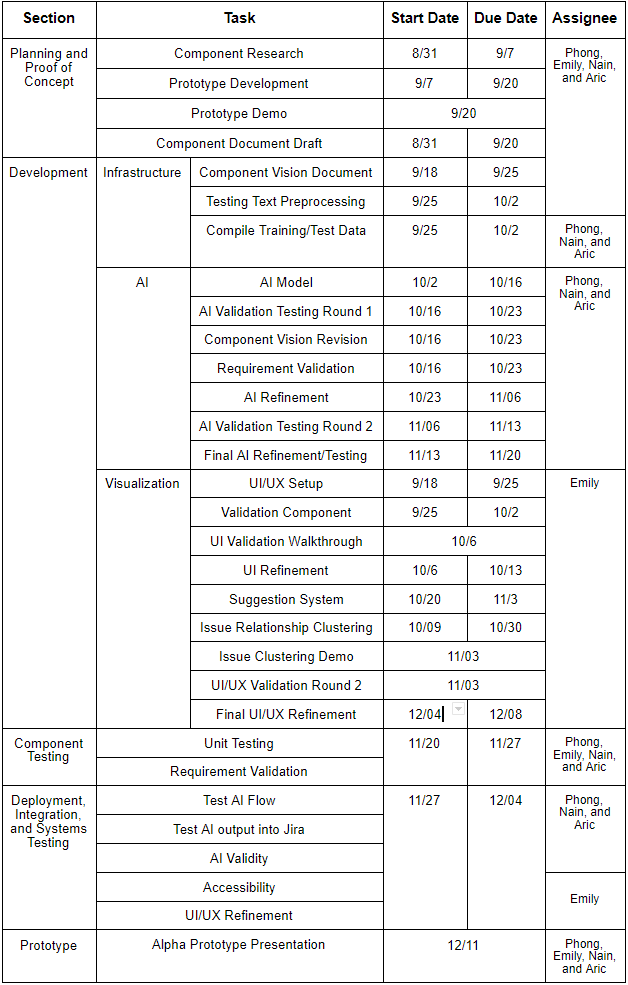
\includegraphics[width=0.9\textwidth,keepaspectratio]{./figure/ProjectTimeline.png}
\caption{Project timeline}
\label{fig:timeline}
\end{figure}

\begin{figure}
\centering
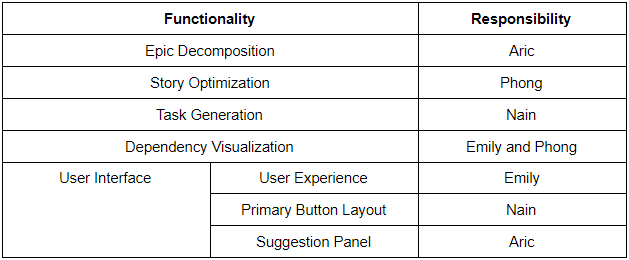
\includegraphics[width=0.9\textwidth,keepaspectratio]{./figure/FunctionResponsibility.png}
\caption{Team member responsibility breakdown}
\label{fig:responsibility}
\end{figure}
%\section{Collaboration}
This project was used as a capstone project. It was given as one of various options that the team could choose for their capstone. The reason this specific project was chosen was because it was intriguing, since none of us had any previous experience in AI and could therefore learn something new and relevant to current industry trends.

For this project we had various people collaborating. The team consisted of 1 faculty advisor, 1 business mentor, 1 faculty mentor, SCORE 2021 prompt sponsor, and 4 undergrads. It was set up to where the business mentor would be the customer, since he already had industry experience. Since this is used as a capstone there are course assignments that needed to be completed this is where the faculty mentor was used for. He provided feedback to make sure the documentation for the project would satisfy course assignments. The faculty advisor assisted with AI components design questions, since he has a background in AI. He was able to provide insightful information on which possible implementations may be needed for the AI components. The prompt sponsor was used to clarify project requirements. One undergrad was assigned the role of team liaison for easier communication between the different people involved.

In the beginning the team was split into two parts AI and UI where the AI components were considered priority. Three undergrads focused on the three requirements needed for the AI which are epic to user story, user story optimization, user stories to tasks and the last one focused on the UI requirements of visualization of their relationships. Later into the project the UI was moved as top priority. The UI consisted of visualizations between the relationships, showing the user suggestions and integrating the new buttons to the Main UI. By breaking up the AI and UI into parts allowed for more efficiency. Each component the undergrads chose was based on what intrigued them the most.

The team met a minimum of 2 times per week to go over documentation that was needed to complete the course and work on implementing the AI components and UI for the project. These meetings would feed into the business mentor meetings that were held once a week. Each time a new implementation piece was completed, it was discussed during the business mentor meetings to receive feedback from a customer perspective.

\begin{figure*}
\centerline{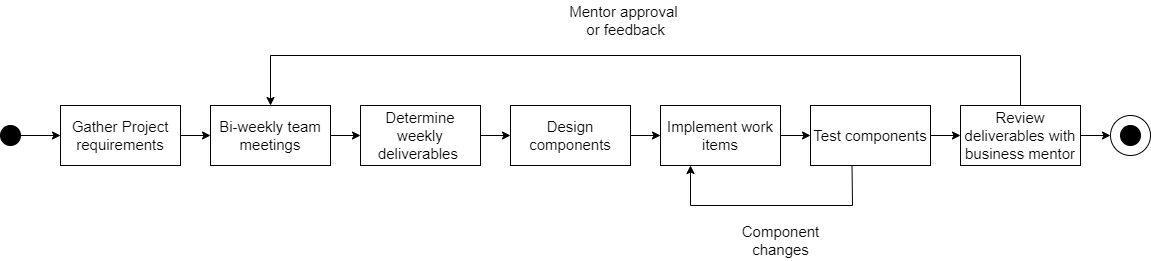
\includegraphics[width=\textwidth,height=\textheight,keepaspectratio]{./figure/ActivityDiagram.png}}
\caption{Activity Diagram outlining the development processes}
\label{fig:ExampleDataFlowDiagram}
\end{figure*}\

In the following sections, we will describe more in detail what work items and deliverables we performed during the project lifecycle.
\section{Requirements}
\label{requirement}

\subsection{Preliminary Analysis}
We first performed analysis on the given proposal in Section \ref{scope}. On the infrastructure side, the proposal requires the project to be integrated into Jira. Among the different versions of Jira software available, the team chose Jira Cloud over Jira Server, for its cloud-based nature is more compatible in modern workplace. 

For the purpose of our project, we consider the following key concepts. 
\textbf{Epic} is defined as a collection or narrative of user stories; they contain more information as to the functional usage of a target project being documented. The next level is \textbf{User Story}, which is a compact set of requirements. These requirements can be further broken down into \textbf{Tasks}, actionable items to be completed as part of a user story. 
Epic, User Story, and Tasks are the three levels of requirements items that our tool focuses on. 

\subsection{Requirement Modeling with KAOS}
First, the team modeled the requirements using KAOS models\cite{KAOS}. KAOS is a Goal-oriented requirement engineering \cite{GOAL} tool that emphasizes goals in requirement acquisition. The team built the KAOS models to guarantee thorough traceability across all requirements, which includes describing the problems, identifying top level goals to address problems and stating the constraint for solutions, etc. Moreover, using the KAOS models, the team could easily remove or add requirements as we encounter new information and changes. The KAOS tutorial handbook \cite{KAOS} also provides universally applicable generic patterns for reference, and we specified our initial goals by adopting these patterns, with selected models presented below.

\begin{figure}
\centering
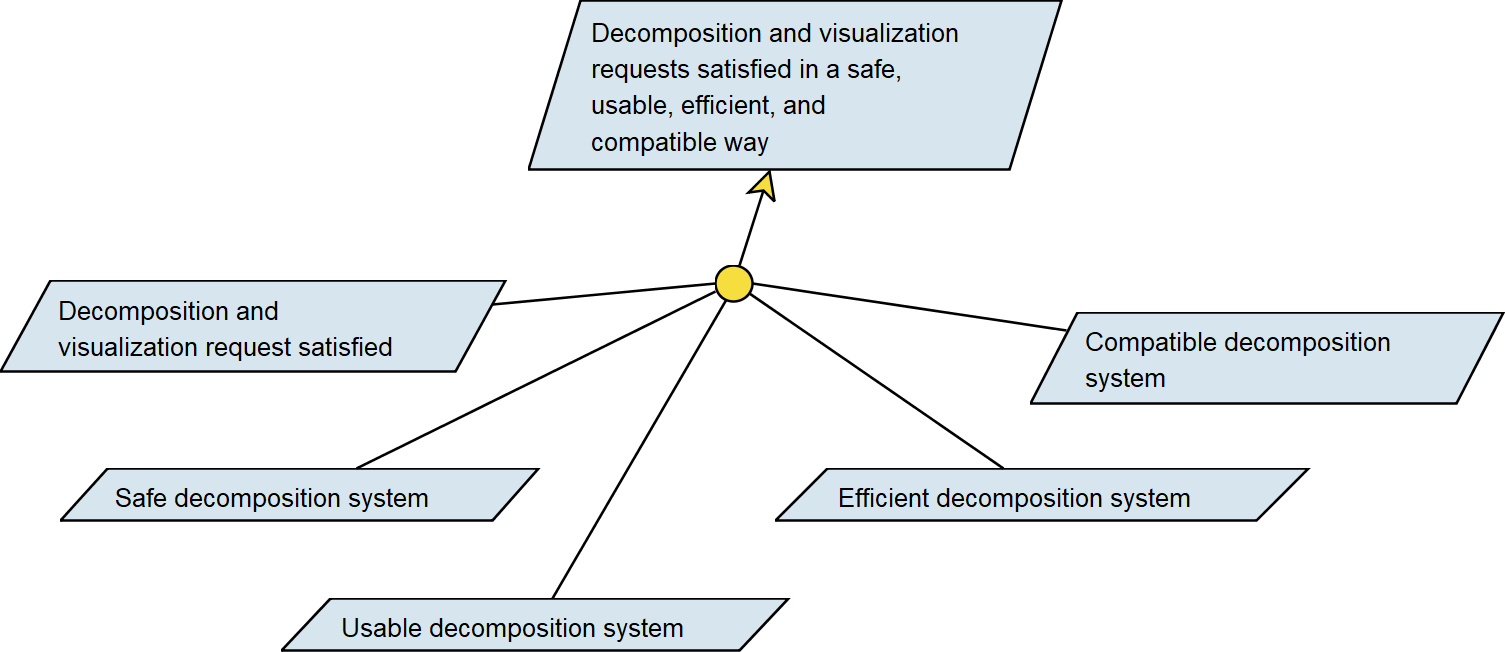
\includegraphics[width=\textwidth,keepaspectratio]{./figure/GoalsNFR1.png}
\caption{Top level goal model of AI4Agile}
\label{goal1}
\end{figure}

We identify three primary processes to handle the requirements items defined above: 1) Epic Decomposition, 2) Story Optimization, and 3) Task Generation. Fig. \ref{goal1} defines the top-level goal for the entire system, with subgoals that enumerate all cases that must be covered to fulfill our main goal. The subgoals each encompasses a portion of the functional and nonfunctional requirements (FRs and NFRs) of the system. As shown in Fig. \ref{goal1}, the goals that our system should achieve are:

\begin{itemize}
	\item Decomposition and visualization request satisfied
	\item Safe decomposition system
	\item Usable decomposition system
	\item Efficient decomposition system
	\item Compatible decomposition system
\end{itemize}

The goals for “Safe”, “Usable”, “Efficient”, and “Compatible System” covered the NFR portion of the system. By using respective generic patterns from \cite{KAOS}, we generated the nonfunctional requirements for our system as shown in Table \ref{nfrs}.

\begin{table}
\centering
\caption{Non-functional requirements}
\label{nfrs}
\begin{tabular}{ |c|c| } 
\hline
\multicolumn{1}{|c|}{\textbf{ID}} & \multicolumn{1}{c|}{\textbf{Description}} \\
\hline
NFR1 & Show resources about Agile development \\
\hline
NFR2 & Follow Agile development process \\
\hline
NFR3 & Have presets for user without domain expertise \\
\hline
NFR4 & Show notification about decomposition status \\
\hline
NFR5 & Do not store information on third-party database \\
\hline
NFR6 & Only query Jira the information that is needed \\
\hline
NFR7 & Software is secure \\
\hline
NFR8 & Retain original sentences in epics with minimal modification \\
\hline
NFR9 & The response time for AI processing is less than five seconds \\
\hline
NFR10 & The response time for visualization is less than two seconds \\
\hline
NFR11 & Visualization only generates important relationships \\
\hline
NFR12 & Available on Atlassian Marketplace \\
\hline
NFR13 & Available on Atlassian Partner Marketplace \\
\hline
\end{tabular}
\end{table}

\begin{figure}
\centering
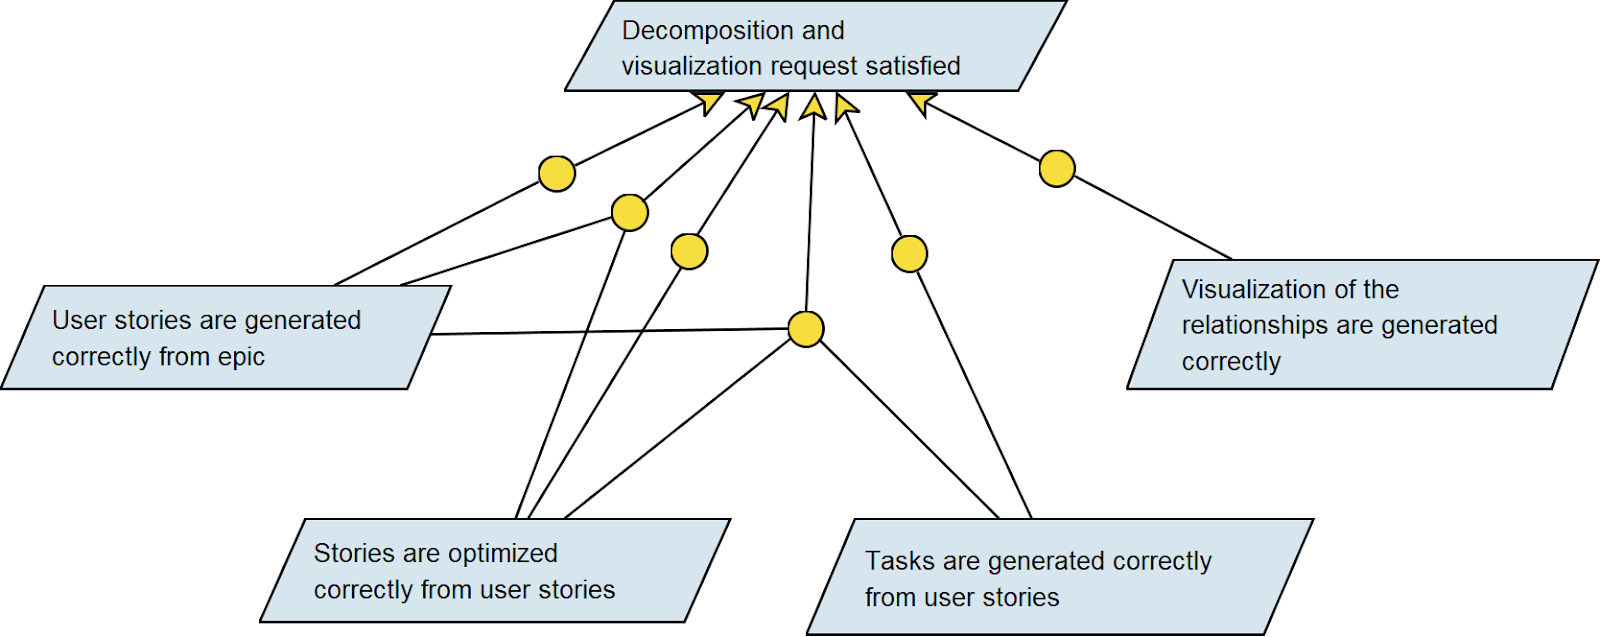
\includegraphics[width=\textwidth,keepaspectratio]{./figure/GoalsNFR2.png}
\caption{Functional goal decomposition continued from Fig. \ref{goal1}}
\label{frgs}
\end{figure}

Next, we broke down the “decomposition request and visualizations satisfied” goal into subgoals, which correlated to the main FRs. Fig. \ref{frgs} shows the first level of functional subgoals, listed below: 

\begin{itemize}
	\item User stories are generated correctly from epic
	\item Stories are optimized correctly from user stories
	\item Tasks are generated correctly from user stories
	\item Visualization of the relationships are generated correctly
\end{itemize}

Each subgoal in Fig. \ref{frgs} has its own KAOS goal models that were further refined. Due to space constraint, we include one example in Fig. \ref{fr1}. Fig \ref{fr1} shows how we refined the subgoal ``User stories are generated correctly from epic'' into the specification. It also identifies the agents responsible for fulfilling this subgoal.  From these models, we obtained the functional requirements as shown in Table \ref{frt}.

\begin{figure}
\centering
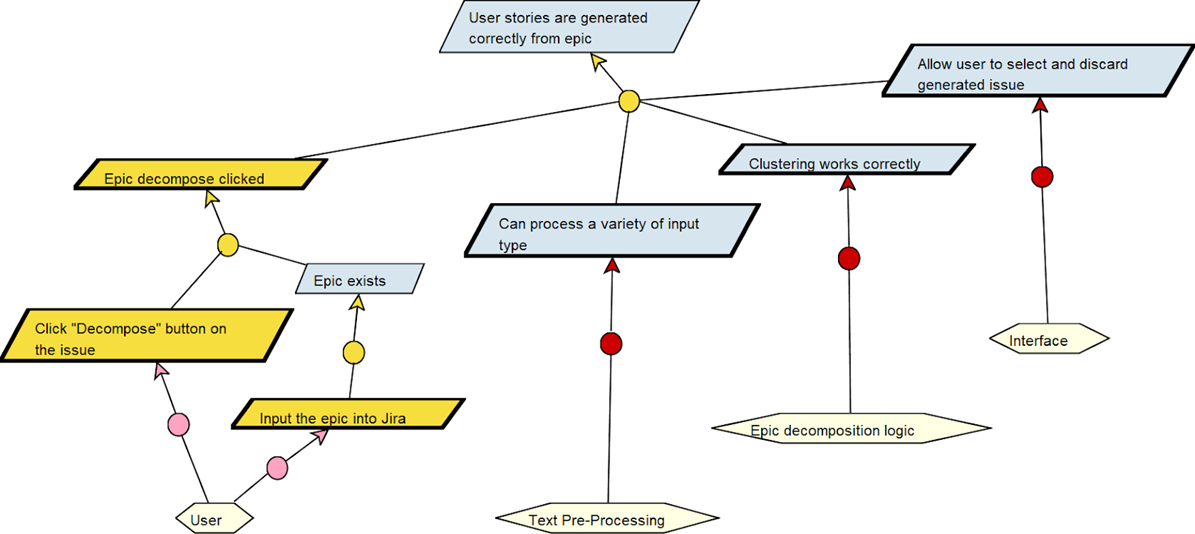
\includegraphics[width=\textwidth]{./figure/GoalsFR1.png}
\caption{Further refinement of one subgoal in Fig. \ref{frgs}}
\label{fr1}
\end{figure}

\begin{table}
\centering
\caption{Functional requirements}
\label{frt}
\begin{tabular}{ |c|c| } 
\hline
\multicolumn{1}{|c|}{\textbf{ID}} & \multicolumn{1}{c|}{\textbf{Description}} \\
\hline
FR1 & Clustering works correctly \\
\hline
FR2 & Allow user to select and discard generated issue \\
\hline
FR3 & Can process a variety of input types \\
\hline
FR4 & User stories extraction works correctly \\
\hline
FR5 & Retain user stories if those are small enough \\
\hline
FR6 & Sentence building works correctly \\
\hline
FR7 & Show the explicit relationship between issues as a tree \\
\hline
FR8 & Show the implicit relationship of developers to the issues as clusters \\
\hline
FR9 & Allow user to show and edit relationship \\
\hline
FR10 & Show a customizable type and depth to relationship between issues \\
\hline
FR11 & The graph should render as the object is selected \\
\hline
\end{tabular}
\end{table}

\subsection{Requirements Summary}
The NFRs and FRs in Tables \ref{nfrs} and \ref{frt} defined the initial scope for our implementation, each with their own specifications developed. To summarize the system's three major functional processes, we concluded that: 1) Epic decomposition means that, given a semi-structured, manually entered epic, the app would refine it into user stories in the form of subject-based clusters; 2) Story optimization further breaks down large stories into smaller stories; 3) Task generation is done by performing part-of-speech analysis on the user stories. 

Furthermore, to satisfy the NFRs such as integrity, for each process, the app would offer suggestion results to the user, allowing them to pick and choose which user stories and tasks to add to their Jira board. The user can further adjust settings, i.e. number of tasks to be generated, to fine tune the granularity of generated results. Finally, epics, user stories, and tasks can be displayed in an interactive tree/cluster graph that shows the explicit and implicit relationships among them.

The project's main motivation is to save time for manual Requirement Engineering (RE). While AI could be used in different ways to achieve this goal, our app predominantly utilized the AI component in text processing, generating increasingly refined results to support an efficient RE process. This approach could also increase the consistency of the RE outcomes, as the central process reduces the impact of human factors. In the meantime, we recognized that knowledge and experiences from a skilled project manager is still crucial, thus we make sure that the tool would not alter or discard any original input, preventing unintended consequences. Last but not least, with direct feedback from our mentor, the team formatted sample requirements we have encountered in practice, and developed the user stories used for demo and verification purposes, as presented in Section \ref{demo}.
\section{Design}
\label{design}

\subsection{AI Selection Criteria}
\label{subsection:criteria}
Performing an epic breakdown involves a combination of clustering related requirements, specifications, and details along with the further breakdown of complex info into smaller stories and tasks. Clustering can be performed in either supervised or unsupervised learning. Supervised learning requires the existence of a data set that has been correctly labeled. Although the team might be able to generate general data set of decomposed epics, we concluded that an typical epic might have too many subjects, and we would not be able to produce any accurately labeled model for training purposes. 

Additionally, for the stated purpose of increasing consistencies, we made the assumption that the decomposition process would not rely upon historical project information, such as previously completed epics or sprints. As a result, unsupervised clustering techniques were chosen as it couldo be equally applicable to new and old projects alike.

The last criteria for the text processing approaches was that we would not attempt to generate ``new'' information based on given input. This was due to the previously discussed lack of data, specific to the project domain, that could be used to potentially generate stories and tasks. Table \ref{table:ai} summarizes the decisions we made regarding the selection of AI techniques.

\begin{table*}[h]
	\caption{AI design choices}
	\label{table:ai}
	\begin{tabularx}{\textwidth}{|p{3cm}|p{3cm}|p{2cm}|X|}
	\hline
	Component & Options & Choice & Reasoning\\
	\hline
	Epic Decomposition & 
	\begin{minipage}{0.15\textwidth}
		\begin{itemize}
		\item KMeans
		\item Meanshift
		\item DBSCAN
		\item OPTICS
		\end{itemize}
	\end{minipage} &
	Mean-shift & All of the mentioned clustering algorithms are dynamic as they do not require the number of clusters as input. Mean-shift only requires the size of the region to search through (bandwidth), which can be estimated, where all other options require arbitrary values to create clusters.\\
	\hline
	Story Optimization & 
	\begin{minipage}{0.15\textwidth}
		\begin{itemize}
		\item TF-IDF
		\item SIF
		\item Word2vec
		\item Cosine simularity
		\item Word mover's distance
		\end{itemize}
	\end{minipage} &
	\begin{flushleft}
	SIF with word2vec and Cosine similarity
	\end{flushleft} & TF-IDF is the most simple for word embedding. SIF with word2vec can achieve a higher accuracy than TF-IDF with the custom word2vec model that is relevant to the topic. WMD is far more expensive to calculate, especially on longer texts. Cosine similarity can give the same performance without losing too much semantic similarity.\\
	\hline	
	Task Generation & 	
	\begin{minipage}{0.15\textwidth}
		\begin{itemize}
		\item Sentence classification
		\end{itemize}
	\end{minipage} & Sentence classification & There is a need to split up the different types of sentences, such as complex and compound, into simple sentences, in order for them to be manipulated into tasks. To do this, sentence classification is the necessary first step.\\
	\hline	
	\end{tabularx}
\end{table*}

\subsection{Epic Decomposition}
Through manual decompositions of epics into stories it was identified that the process fundamentally involved the categorization of requirements and specifications. From such, text clustering techniques based upon the vectorization of the contents of epics. Each requirement, assumed to be in the form of a complete sentence or distinguishable section, is vectorized and normalized so a comparison can be performed.

Based on a series of tests on a simpler text clustering problem, K-means, a non-deterministic centroid-based clustering technique, yielded the best results when it came to creating consistent clusters of requirements. The downside to K-means is that it requires the number of clusters to be identified, forcing there to be user input or an estimation to be made. Since it was a goal to have the app be applicable to a large range of epics, in terms of topic and size, issues such as DBSCAN, OPTICS, and Mean shift were explored as they are dynamic and do not require the number of clusters to be specified. DBSCAN/OPTICS are density-based clustering techniques and Mean shift is a centroid-based clustering technique. Ultimately, it was decided to go with Mean shift since the implementation of the technique included an estimation of the cluster sizes, thus requiring no external input.

\subsection{Story Optimization}
Story optimization is further breaking down a story to if it contains more than one story or software feature that needed to be achieved. For story optimization, sentence similarity is high priority. 

A pre-trained Word2Vec model was used to extract the features out of sentences. A sentence embedding technique called SIF embeddings (Smooth Inverse Frequency) was used to compute sentence embeddings as a weighted average of word vectors. Using the features, a comparison was made by calculating the cosine similarity between sentences. 

The result was the similarity coefficient between sentences and it could be used to group sentences together based on their degree of similarity. A function decision was implemented to correctly group sentences from the similarity coefficient using a specified threshold level. 

\subsection{Task Generation}

Task generation was identified as the process of breaking down a requirement into its most simplest form. Based on the criteria laid out in Section \ref{subsection:criteria}, simplification on the existing input of requirements could be completed by deconstructing complex sentences into simple sentences. 

The first process to break down sentences was to use parts-of-speech tagging to remove any unnecessary words from the sentence; this was done by identifying stopwords, since simple sentences contain only one subject and predicate. Therefore, using the word dependency we were able to determine which words were connected to the subject. By making sure the sentence contained one subject and verb we were able to create a complete simple sentence. Everytime a new subject was found that meant a new sentence was needed. Each simple sentence generated from the stories can then be suggested as tasks.

\subsection{Process Flow}

\begin{figure*}
\centerline{\includegraphics[width=\textwidth,height=\textheight,keepaspectratio]{./figure/ExampleDataFlowDiagram.png}}
\caption{Simplified Data Flow diagram outlining the flow of the decomposition processes}
\label{fig:ExampleDataFlowDiagram}
\end{figure*}\

There is an overall linear flow, as seen in Figure \ref{fig:ExampleDataFlowDiagram} to AI4Agile’s main processing: Epic Decomposition, Story Optimization, and then Task Generation. Additionally, the relationship graph may be generated at any point and is independent of the previously mentioned flow. It is possible that the starting point in the flow may vary between uses. For example, a user may have manually entered in all their overarching user stories for their epic, forgoing the use of the Epic Decomposition process. From these entered stories, either story optimization or task generation may be performed.

\begin{figure*}
\centerline{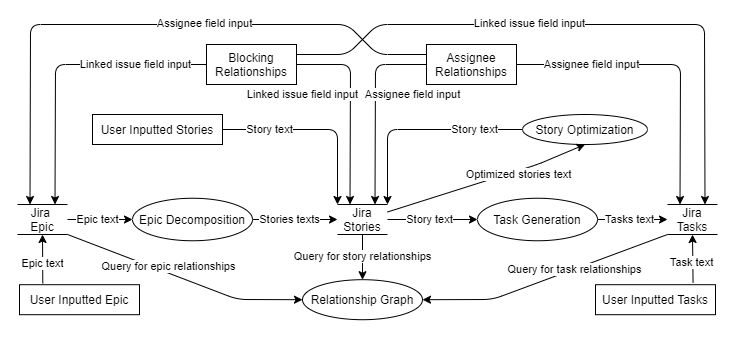
\includegraphics[width=\textwidth,height=\textheight,keepaspectratio]{./figure/DataflowDiagram.png}}
\caption{Data Flow diagram showing the various entry points, sources of data, and processes within Jira and AI4Agile}
\label{fig:DataFlowDiagram}
\end{figure*}
Placeholder cause I need to reference Figure \ref{fig:DataFlowDiagram}
\subsection{Relationship visualization}
The purpose of the relationship graph is to give users a visual representation of the dependencies between a selected issue in Jira and the issues that are related to it. Currently in Jira, hierarchies are shown minimally in such ways as dropdown lists from epics, or lists within an issue selection pane of either children or explicitly specified blocking/cloning/similarity relationships. This graph provides a way to view those relationships in one place at a glance, for ease of visual understanding.
\subsection{User Interface and Experience}
For the user interface and experience, a combination of prototyping and stakeholder meetings went into the decisions displayed in Table \ref{tab:UIUXDesignChoices}. The highest priority was to make the interface as intuitive and easy to use as possible, to fall in line with the larger project goal of saving users time throughout the agile development process.
\begin{table*}[h]
	\caption{UI and UX Design Choices}
	\begin{tabularx}{\textwidth}{|p{3cm}|p{3cm}|X|}
	\hline
	Options & Choice & Reasoning\\
	\hline
	\begin{itemize}
		\item Suggestion Format
		\item Chatbot
	\end{itemize} &
	Suggestion format & A conversation element can slow down the process and ease of use. A suggestion format was chosen to avoid the case where using the plugin as one who is familiar with the project and decomposition methods would slow down a decomposition process instead of accelerating it.\\
	\hline
	\begin{itemize}
		\item Templated epic input
		\item Unrestricted epic input
		\item Semi-structured epic input via guidelines
	\end{itemize} &
	Semi-structured epic input via guidelines & A template was deemed too restrictive and time consuming for the user, but unrestricted input was infeasible for AI processing. Thus, the choice was to present the user with guidelines in the user manual for what the optimal structure of an epic would be for use with this plugin.\\
	\hline	
	\begin{itemize}
		\item External database use
		\item Strictly Jira database use
	\end{itemize} & 
	Strictly Jira database use & There is a need to split up the different types of sentences, such as complex and compound, into simple sentences, in order for them to be manipulated into tasks. To do this, sentence classification is the necessary first step.\\
	\hline
	\begin{itemize}
		\item Relationship Graph as tree
		\item Relationship graph as clusters
		\item Relationship graph as tree and clusters
	\end{itemize} & 
	Relationship graph as tree and clusters & While the original concept had the relationships as clusters, it was determined from stakeholder input that a tree format would likely be more intuitive to the user base. At the same time, if the relationships to be shown are only developer assignments, the lack of parent-child relationships suggested clustering was still the sensible choice.\\
	\hline
	\begin{itemize}
		\item Undo functionality for story/task creation
		\item Preview button for story/task creation
		\item Iterative creation process
	\end{itemize} & 
	Iterative creation process & With undo functionality, there were issues such as where it would make sense to have such a thing, how far after the action it should be able to be undone, and how much additional effort would be needed to implement it. The reasoning behind this feature in general was for new users to be able to experiment with the plugin without fear of consequences. It was determined that switching to an iterative process, where users can create one story or task at a time from the suggestions, would serve this same purpose to lessen potential consequences and still allow users to experiment. As a result of the iterative creation process, the need for a preview system was eliminated.\\
	\hline
	\end{tabularx}
\label{tab:UIUXDesignChoices}
\end{table*}
\section{Implementation}
\label{implementation}

The AI4Agile app was implemented within Jira Cloud as an app and connected to a Python-based backend.

\subsection{Frontend}
As part of the Atlassian Design Guidelines \cite{jira3}, a frontend library, Atlassian User Interface (AUI) \cite{jira4}, is provided to create new UI elements to match Jira’s style and user experience. The team coded our own UI components adhering Design Guidelines from Atlassian.

Within Jira, all objects (epics, stories, issues) are rendered in the same way, each containing a shared issue panel as shown in Fig. \ref{fig:issueView}. Our app is implemented within the issue panel in the form of additional panels that can be opened through added buttons. When a process button or visualization button is pressed, a new panel appears.

Each of the processes uses the same suggestion panel, with variations depending on the need for user inputs in the case of epic decomposition and story optimization. The suggestion panel, when opened, requests suggestions from the backend through jQuery AJAX \cite{ajax} and displays a loading animation until the suggestions are received. Stories can be changed and once checked, they can be created which is done by passing the selected stories via an AJAX call to the backend. The responsibility to populate selected stories to the Jira board is handled by the backend.

\begin{figure}
\centering
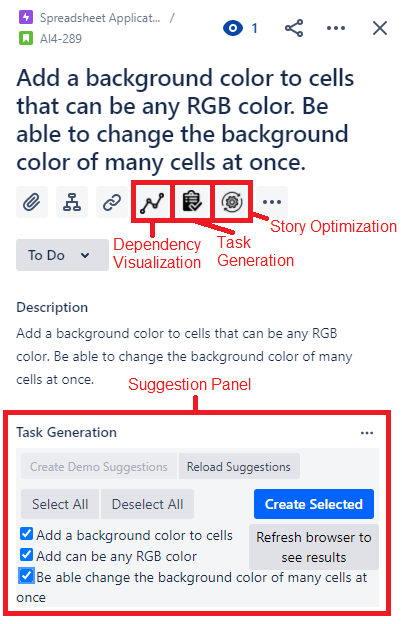
\includegraphics[width=.5\textwidth,keepaspectratio]{./figure/Frontend.png}
\caption{Issue Panel within Jira with Task Generation suggestions }
\label{fig:issueView}
\end{figure}

\subsection{Backend}

The backend served two primary purposes: generating suggested issues and populating selected suggestions into Jira. Each process has its corresponding suggestion generator and selected suggestion creator since the specifics of each type of issue varies. Jira handles all issue types (i.e. epics, stories, and tasks) the same, each having the same set of shared fields with the addition of custom fields depending on the type of issue.

All three processes were implemented using available Python libraries, with the primary interface also written in Python. The interface uses Flask \cite{flask}, a Python web framework, to receive messages sent by AJAX in the frontend. The information needed from the issues are gathered by querying the Atlassian Rest API \cite{jira5} through “atlassian-Python-api” \cite{jiraPython}, which simplifies Atlassian API calls. When generating suggestions, the description is queried for and passed as a list of individual requirements to the text processor. Suggestions are then passed back through a reply to the original message. Once a user selects, and possibly edits, which issues they would like to have populated in their Jira board, then the original issue is queried again to percolate existing fields, such as assignee, reporter, due date, tags, or sprints, to the newly created child issues. Each newly created issue is given a blocking relationship to the issue they were derived from. For example, all the created stories from an Epic Decomposition will “block” the epic from being completed. Any further tasks created from Task Generation on a story will “block” the story from completion.

\subsubsection{Epic Decomposition}
The Epic Decomposition process was implemented using k-means clustering over a dynamic clustering technique, such as DBSCAN or Mean shift. Dynamic clustering techniques were unable to be implemented in a manner that yielded consistent meaningful clusters across many epic inputs. This was a result of an inability to filter noise such that the clusters were neither completely disjoint nor entirely overlapping. Thus, K-means, a centroid-based clustering algorithm, was used at the cost of selecting a default number of stories to generate. The default number of stories generated is five, but the user can select between two and ten stories using a newly added slider in the UI for the Epic Decomposition process.

\subsubsection{Story Optimization}
For Story Optimization, the process maintained the initial implementation without any significant changes to the algorithm. The algorithm utilizes a pre-trained Word2Vec model, along with SIF and cosine similarity functions from the scikit-learn python library. Initially, the degree of connectivity between sentences was specified by choosing the optimal threshold level. However, it was changed so that the user can choose to increase or decrease the degree of connectivity between sentences offering more flexibility in the generated results.

The user can choose to increase or decrease the degree of connectivity between sentences. The slider displays options from 0 to 10, which maps to values from 0.65 to 0.75 as threshold values on the backend. The slider integration was a feature that was added based on mentor feedback. A parameter is exposed to give the user more control of the output. The exposed parameter is the degree of connectivity between the sentences. It was determined after impact analysis that it is better to implement it this way because it generates more meaningful results tailored to each user. This also eliminates the need for having a fixed threshold number, since the optimal threshold number can vary between inputs.

\subsubsection{Task Generation}
The approach for Task Generation was based off a decomposition approach by Das, Majumder, and Phadikar in 2018\cite{NLP1}. Initially the natural language toolkit (NLTK) library was selected for implementing task generation, but it lacked the need for parts-of-speech tagging. The main feature that NLTK lacked was word dependency. Word dependency is important to this process, since this was the main feature used to create simple sentences. Word dependency returns a pair of words, identifying the dependency between the two. The new Python library being used is Stanza. This library allows for parts-of-speech tagging, word dependency, and tree parsing. By having part-of-speech tagging and word dependency, the creation of simple sentences from complex and compound sentences was easier to implement.

\subsection{Communication}
\begin{figure}
\centering
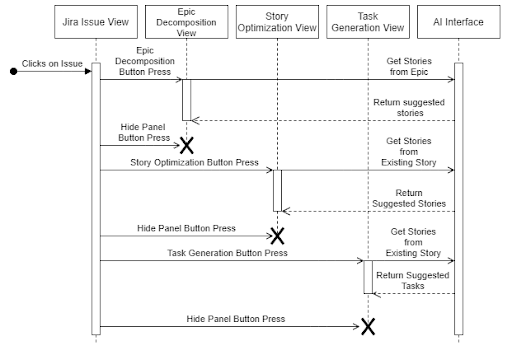
\includegraphics[width=0.75\textwidth,keepaspectratio]{./figure/SequenceFlowDiagram.png}
\caption{Suggestion web panel sequence diagram of messages between the frontend Jira web page and AI4Agile backend}
\end{figure}

The plugin communicates from Jira to the backend interface via a listener through AJAX calls which are received by Flask. When a web panel is opened for any of the three processes, a message is sent to generate and return the suggestion issues. The Jira panel will function asynchronously with a loading animation appearing until the resulting suggestions are received. Once the results are received, populated in the suggestion box, and the desired suggestions are selected by the user, then a message is sent containing which suggestions to then create within Jira.

%\begin{center}
\begin{table}
\centering
\caption{Components, subcomponents, and sources used for implementation of subcomponents}
\begin{tabular}{ |c|c|c| } 
\hline
\multicolumn{1}{|c|}{\textbf{Component}} & \multicolumn{1}{c|}{\textbf{Subcomponent}} & \multicolumn{1}{c|}{\textbf{Source}} \\
\hline
Epic Decomposition & K-means clustering & scikit-learn: machine learning in Python \cite{scikit} \\
\hline
\multirow{4}{*}{Story Optimization} & Word embedding & Google Word2Vec Pre-trained Model \cite{googleword2vec} \\ 
\cline{2-3}
& Feature Extraction & scikit-learn: machine learning in Python \cite{scikit} \\ 
\cline{2-3}
& Cosine similarity & scikit-learn: machine learning in Python \cite{scikit} \\
\cline{2-3}
& Function decision & N/A \\ 
\hline
\multirow{2}{*}{Task Generation} & Sentence classification & Stanford CoreNLP \cite{NLP1} \\ 
\cline{2-3}
& Part of speech tagging & Natural Language ToolKit \cite{nltk} \\ 
\hline
\multirow{3}{*}{UI} & Tree relationship graph & Cytoscape \cite{cytoscape} \\ 
\cline{2-3}
& Clustered relationship graph & Cytoscape \cite{cytoscape} \\ 
\cline{2-3}
& Jira Cloud frontend & Atlassian Connect Express Modules \cite{jiraconnect}\\ 
\hline
\end{tabular}
\end{table}
%\end{center}
\section{Demonstration and Testing}
\label{demo}

\subsection{Demonstration by User Story Walkthrough}

This section describes a walkthrough of two user stories the team developed based on our requirements, to demonstrate the primary features currently implemented in the finished prototype system. 

\subsubsection{Complete Decomposition Use Case}
\label{Scenario1}

\begin{figure}
\centering
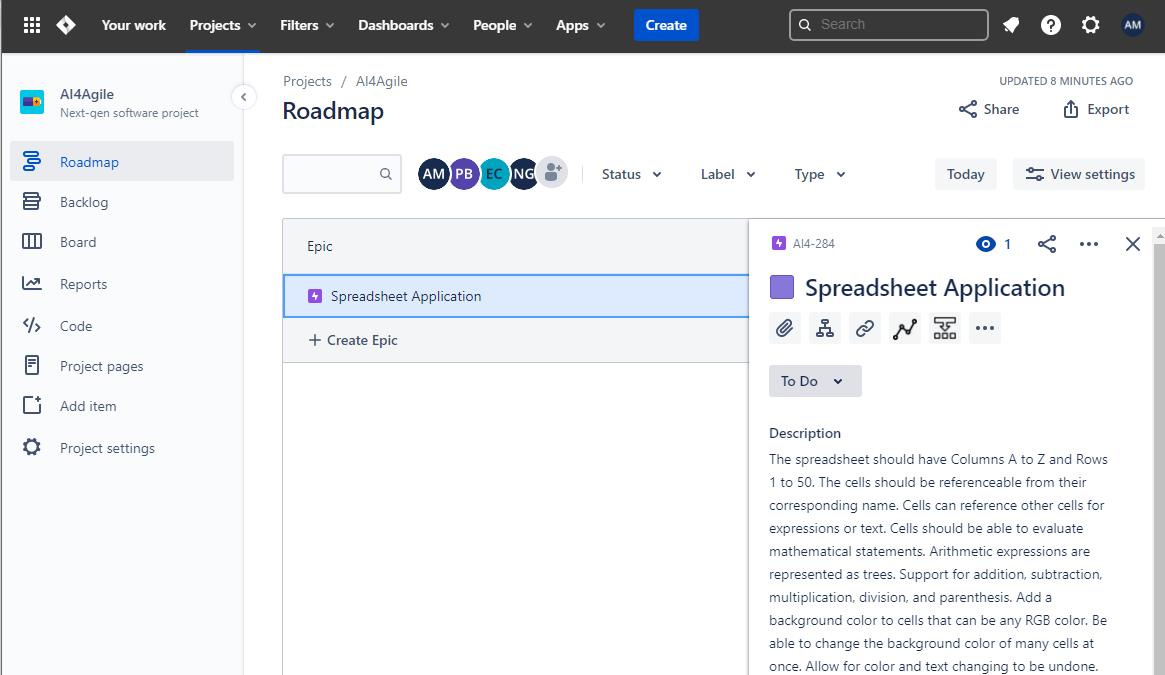
\includegraphics[width=\textwidth,keepaspectratio]{./figure/Scenario1Figure1.png}
\caption{Overall view of Jira Roadmap with Decompose Epic button in focus}
\label{fig:Scenario1Figure1}
\end{figure}

Frank is a software requirements analyst, and he wants to speed up the process of breaking an epic full of requirements into smaller user stories. For this purpose, he installs the AI4Agile plugin to Jira. Frank creates a new epic, puts the requirements for his Spreadsheet Application in as plaintext sentences, and clicks the Decompose Epic button (Fig. \ref{fig:Scenario1Figure1}).

\begin{figure}[ht]
\begin{subfigure}{.5\textwidth}
\centering
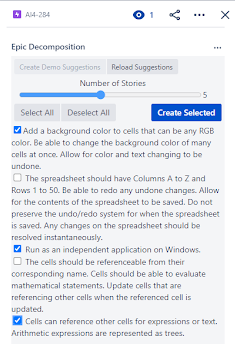
\includegraphics[width=.8\linewidth,keepaspectratio]{./figure/Scenario1Figure2.png}
\caption{Generated User Story Suggestions}
\label{fig:Scenario1Figure2}
\end{subfigure}
\begin{subfigure}{.5\textwidth}
\centering
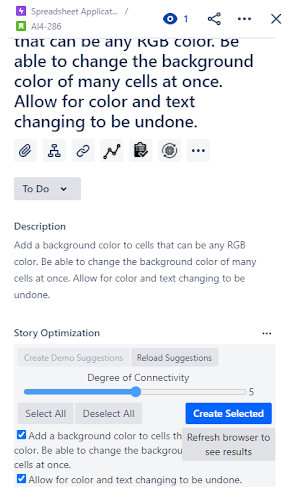
\includegraphics[width=.8\linewidth,keepaspectratio]{./figure/Scenario1Figure3.png}
\caption{User Story Optimization Suggestions}
\label{fig:Scenario1Figure3}
\end{subfigure}
\caption{User Story Suggestions Views}
\end{figure}

Now, Frank looks at the suggestions the AI came up with (Fig. \ref{fig:Scenario1Figure2}). If he decides he does not want to use any of these suggestions, he can click the righthand side ellipsis dropdown to hide the Epic Decomposition panel. If Frank wants more or fewer stories, he can adjust the value on the slider and it will refresh the results. To edit a story, he can click on its text box, then save or cancel those edits. To ignore a story suggestion entirely, he can leave its box unchecked. Once Frank is happy with his resulting user story or the set of stories he wants, he clicks Create Selected. 

After refreshing the webpage, the newly created user stories that Frank approved are visible under the heading of the Spreadsheet Application epic.

If Frank wants to continue the process of breaking up epics, he can go into one of the user stories and click Optimize User Story (Fig. \ref{fig:Scenario1Figure3}). Depending on the size of the user story already, it might be broken down into multiple smaller stories, or left alone if it’s already optimized.

Once the Story Optimization Suggestions are generated, Frank has the same options as with the previous stories: to select or deselect stories via the checkboxes, make edits, or ignore all suggestions. In addition to those options, Frank can choose to adjust the connectivity slider to change how closely related items need to be to stay with the same story.  

Now there are five user stories since the fourth Story was optimized into two separate stories. To continue the decomposition process, Frank opens a story and clicks Generate Tasks (Fig. \ref{fig:Scenario1Figure4}).

\begin{figure}
\begin{subfigure}{.5\textwidth}
\centering
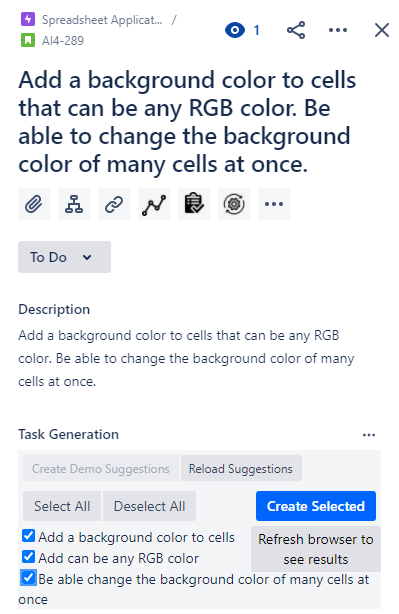
\includegraphics[width=.8\linewidth,keepaspectratio]{./figure/Scenario1Figure4.png}
\caption{Task Suggestions page}
\label{fig:Scenario1Figure4}
\end{subfigure}
\begin{subfigure}{.5\textwidth}
\centering
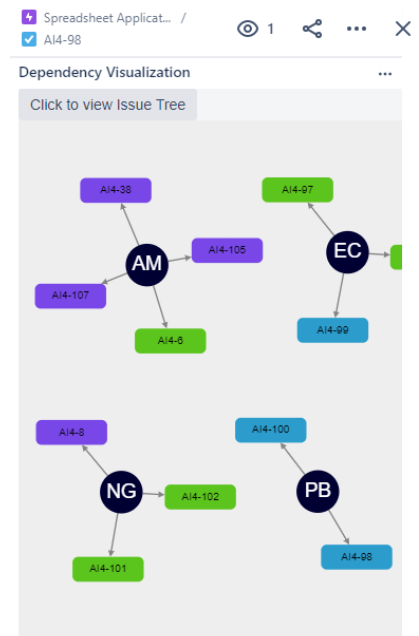
\includegraphics[width=.8\linewidth,keepaspectratio]{./figure/Scenario2Figure2.png}
\caption{Developer cluster graph on a selected task}
\label{fig:Scenario2Figure2}
\end{subfigure}
\caption{Task suggestions and Cluster Graph}
\end{figure}

As before, the options include selecting or deselecting individual suggestions, editing, and ignoring all suggestions. Once he’s happy with the tasks, he clicks Create Selected.

\begin{figure}
\centering
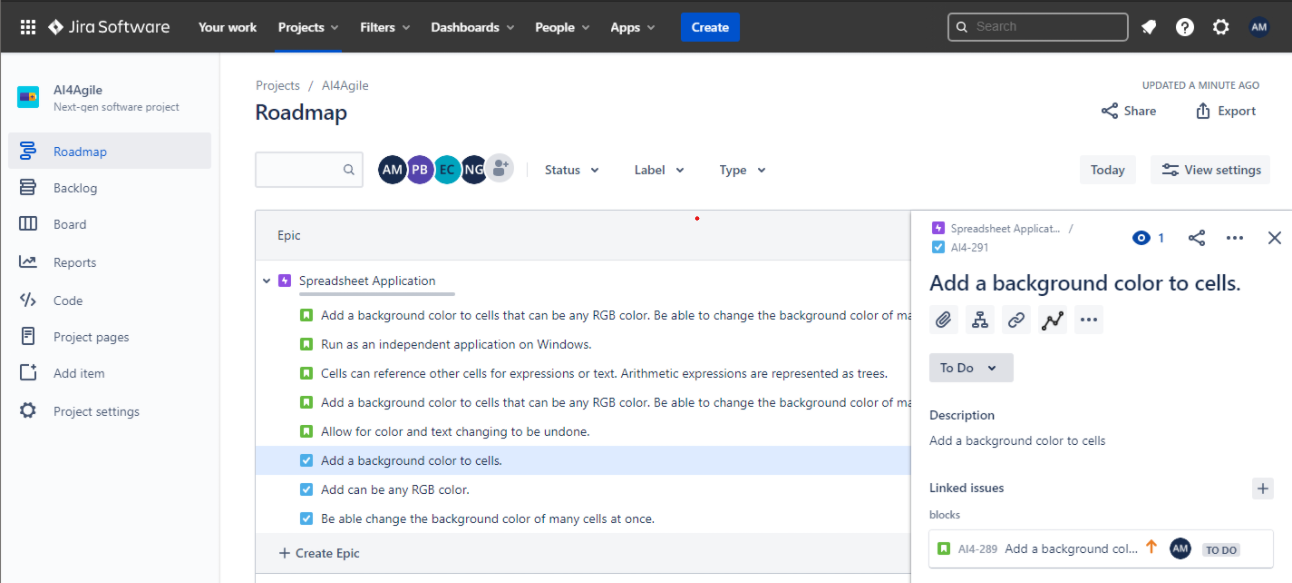
\includegraphics[width=\textwidth,keepaspectratio]{./figure/Scenario1Figure5.png}
\caption{View of newly created tasks for one fully decomposed user story}
\label{fig:Scenario1Figure5}
\end{figure}

The tasks have now been created and linked to their parent story to indicate a blocking relationship. All Frank had to do was make some decisions and maybe edits, and now he’s got one story fully decomposed (Fig. \ref{fig:Scenario1Figure5}).

\subsubsection{Relationship Visualization Use Case}
\label{Scenario2}

\begin{figure}
\centering
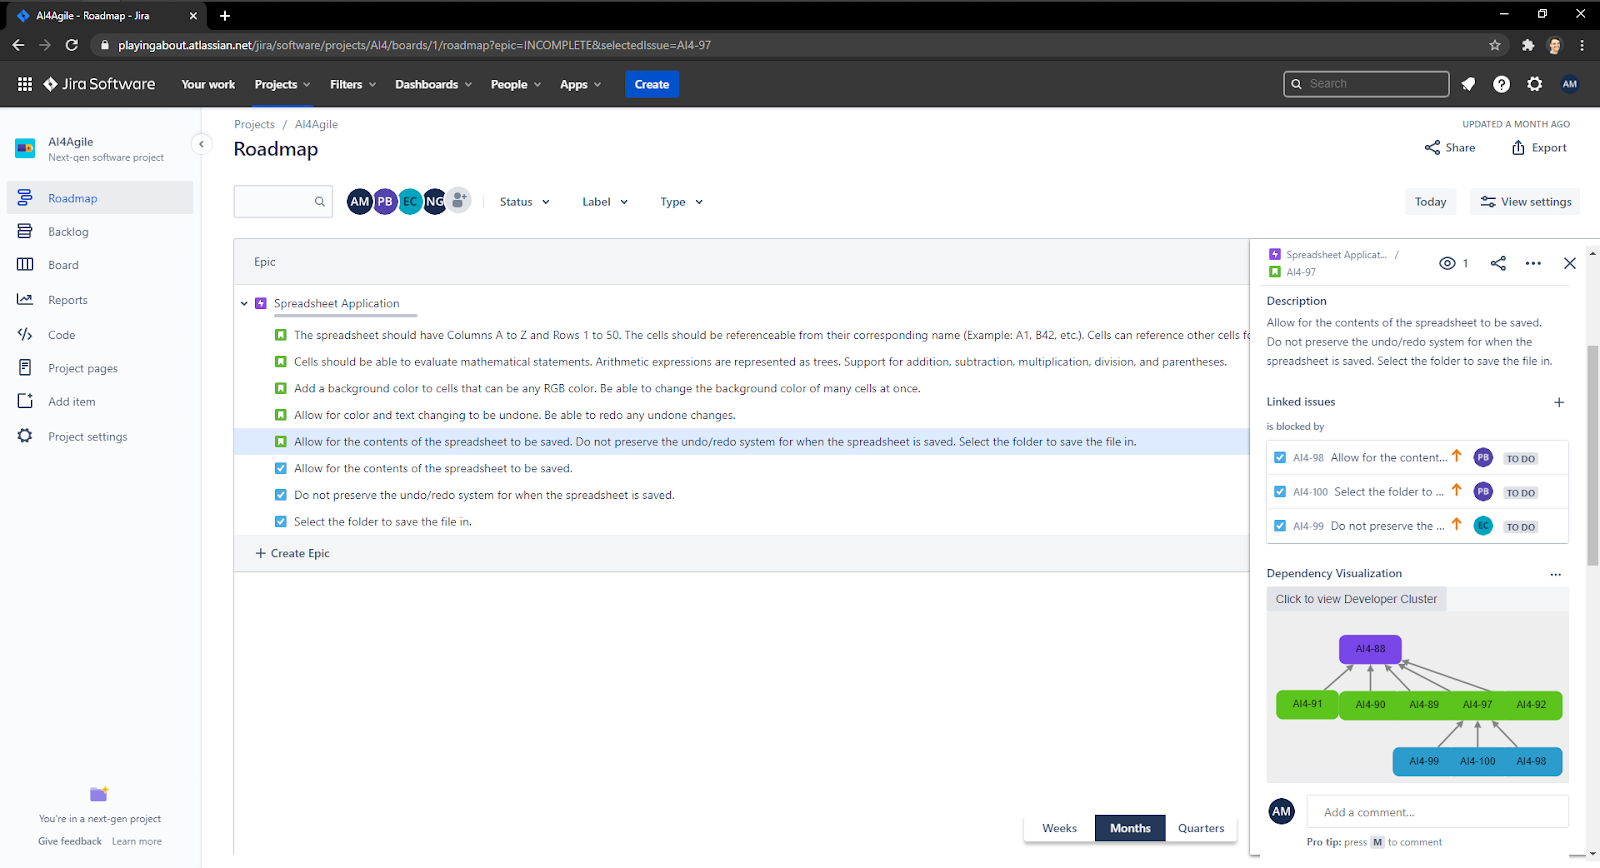
\includegraphics[width=\textwidth,keepaspectratio]{./figure/Scenario2Figure1.png}
\caption{A zoomed out view of navigating to the issue relationship graph}
\label{fig:Scenario2Figure1}
\end{figure}

Madison is a scrum master, and she wants to take a closer look at some of the tasks to make sure the developer assignments make sense. To do this, she uses the AI4Agile Issue Relationship Graph feature by navigating to a certain epic, user story, or task, and finding the graph portion (Fig. \ref{fig:Scenario2Figure1}). Now, Madison can see all the available relationships between the task she has selected and other tasks, stories, and the epic they came from. She is better able to decide whether the team members she assigned to these pieces make sense given the relations between them.

For an alternate view of the relationships, Madison can use the Click to view Developer Cluster button (Fig. \ref{fig:Scenario2Figure1}) to see what the current assignments and workload look like for her team (Fig. \ref{fig:Scenario2Figure2}). To see the previous graph type, she can Click to view Issue Tree button is in the top left.

\subsection{Demonstration by Video and Source Code}
A video demonstration of the functioning AI4Agile application can be found here: \url{http://www.youtube.com}. Additionally, the source code and documentation for this project has been made available at this address: \url{https://github.com/AricMonary/AI4Agile/tree/submission}.

\subsection{Testing}

The application is primarily composed of individual web panels integrated into Jira’s existing UI. As a result, each web panel was able to be created, tested, and reviewed independently from Jira Cloud. The isolation was used to conduct input and output testing, but the modules were generally tested within the context of Jira to ensure that the user experience is seamless between our integrated app and the existing Jira Cloud platform.

The rest of functional testing was performed on component and integration levels. Component testing was separated into two categories: text processing and relationship visualization.

We based the testing of the text processing component upon results from three categories of inputs: ideal, disjoint, and semi-ideal. Ideal inputs were those where all information belonged to clear categories. Disjoint inputs were those where all information fell completely within separate categories. Semi-ideal inputs had both outlier pieces of information and information that distinctly can be clustered with other info. Disjoint inputs were used to evaluate edge case usages of the tool. To represent the average case, semi-ideal inputs were used since natural language understanding from a vector perspective is ambiguous without context.

For integration testing, all possible user paths were explored as each text process could be done independently or sequentially. For example, a user can complete the entire process by entering by decomposing an epic, optimizing the generated stories, and then generate tasks from the optimized stories. However, a user may choose to only optimize stories that were manually entered and then go on to generate tasks from the optimized stories. 

%\section{Verification and Validation}

\subsection{UI/UX Feedback}

The application is primarily composed of individual web panels integrated into Jira’s existing User Interface. As a result, each web panel was able to be created, tested, and reviewed independent from Jira Cloud. The isolation was used to conduct input and output testing but the modules were generally tested within the context of Jira to ensure that the user experience is seamless between our integrated app and the existing Jira Cloud platform.

\subsection{Testing}

Testing was performed on a component and integration level. Component testing was separated into two categories: text processing and relationship visualization.

Text processing component level testing was based upon results from three categories of inputs: ideal, disjoint, and semi-ideal. Ideal inputs were those where all information belonged to clear categories. Disjoint inputs were those where all information was completely separate each with separate categories. Semi-ideal inputs had both outlier pieces of information and information that distinctly can be clustered with other info. Disjoint inputs were used to evaluate edge case usages of the app. To represent the average case, semi-ideal inputs were used since natural language understanding from a vector perspective is ambiguous without context.

At an integration level, all possible user paths were explored as each text process could be done independently or sequentially. For example, a user can complete the entire process by entering by decomposing an epic, optimizing the generated stories, and then generate tasks from the optimized stories. However, a user may choose to only optimize stories that were manually entered and then go on to generate tasks from the optimized stories. 

\section{Future Works and Conclusion}
\label{conlcusion}
As part an academic capstone project, regardless of whether the team would advance into the next stage with the SCORE competition, we plan to continue on with the project for the next few months. The team has so far defined a vision with loose deliverables in mind, and with the goal of finding potential real customers for the tool. Some of the directions we are interested in exploring is included below. 

For this next phase, we will deploy the project to the Atlassian Marketplace, hence also collecting feedback from potential actual customers, which will be helpful for further improvements.  
At the meantime, the team have noticed several possible improvements for our main features. For instance, in the epic decomposition process, we might implement dynamic clustering of stories, that automatically adjust the numbers of stories generated, instead of relying on user provided parameters. The main improvement for story optimization would be in optimizing the algorithm to be faster, as the current wait time is relatively long compared to our goal, as it caused a noticieable significant delay. 

We are also looking into switching from the current supporting package in Java, to the Stanza Natural Language Processing (SNLP) \cite{NLP1} package in Python. The SNLP package has a word dependency feature that could improve the results of task generation, especially in generating complete sentences rather than fragments. The relationship visualization component also has multiple adjustments that could be made, such as filtering and ease-of-use controls for zooming and panning. 

In conclusion, the team has completed the tasks within the scope of we defined based upon the AI4Agile project proposal. In this paper, we presented the team's structure and SE process, as well as all major stakeholders invovled. We then described in details the lifecycle throughout the project, covering requirements, design, implementation and final user story based testing and demonstration. The team have plans to continue the project in the near future as part of our capstone project, and will look into explore several directions where improvements on the main features could be done. The ultimate goal of the team is to deploy the project to be adopted by potential real clients. 
%\section{Conclusion}
This document is used to describe the actions taken to complete the SCORE 2021 AI4Agile prompt on the Jira Cloud platform by building a plugin using the interface and development tools that the parent company, Atlassian, provided. The new plugin performed epic decomposition, story optimization, task generation, and relationship visualization for various forms of user stories. To implement these new features on Jira Cloud, research was done on how Jira Cloud worked, and how the AI components should function and interface with Jira. Determining the best area to implement the new features was important, because the team wanted somewhere the user frequently visits and which can be seen easily. Section 6 of this paper went into detail on the specific area chosen and its reasoning. 

The team for this project consisted of 7 people, including mentors and advisors, where only the faculty advisor had previous knowledge of AI, therefore the rest of the team members had a steep learning curve. Due to the wide range of AI types, research needed to be done to determine the best AI type for each component. The specific AI type for epic decomposition uses K-means clustering, while story optimization uses a combination of word embedding, feature extraction, and cosine similarity. For task generation, part-of-speech tagging and sentence classification were used. Section 6 explained the implementation details of these components, while section 5 went into the rationale behind the sub-components used. In the end, connecting the backend processes into Jira Cloud required learning to use another set of tools, namely Flask and jQuery AJAX, which were also mentioned in section 6. 

Overall, the AI and UI components performed well, but could be improved. For example, task generation results would not always be complete sentences, creating a need for editing the suggestions before use. This potential for improvement is where the future works in section 9 come in, as they fall into the plans for the next phase of development.

\section*{Acknowledgment}
Special thanks to Dr. Hoa Khanh Dam, Dr. Bolong Zeng, Prof. Jeremy Thompson, and Skip Baccus for their support, assistance, and time given to the team and this project.

\bibliographystyle{plain}
\bibliography{ref}

\end{document}
